\documentclass{ctexart}
\usepackage{graphicx}
\usepackage{subfigure}
\usepackage{hyperref}
\usepackage{subfigure}
\usepackage{geometry}
\geometry{left=2.5cm,right=3.5cm,top=2.5cm,bottom=2.5cm}
\CTEXsetup[format+={\flushleft}]{section}

\begin{document}
\CJKfamily{li}
\title{周报}
\author{刘精昌}
\maketitle

\fangsong
\section*{本周工作}
    这周主要调研了Gauss process、kernel相关。
\begin{enumerate}
  \item 看了MLAPP第14、15章的部分内容,分别介绍了kernel和Gauss Process。
  \item 看了一篇tutorial《Gauss Processes in Machine Learning》以及一份presentation《Multiple Kernel Learning》。
  \item 论文《Structure Discovery in Nonparametric Regression through Compositional Kernel Search
David》ICML13,该文提出了Compositional Kernel,Compositional Kernel由base kernel组成。base kernel示意图及其描述的时间序列形状如图 1 所示。base kernel简单组合(加、乘)具有一定的可解释性。base kernel简单组合示意图及其描述的时间序列形状如图 2所示。 Time Series可由GP来描述,选择GP中的Compositional Kernel,再依照加性,对其分解成简单的base kernel组合,于是可以发现Time Series的结构,如图 3 所示。图3中Compositional Kernel为$SE × ( Lin + Lin × ( Per + RQ ) )$,可分解成$SE × Lin$、$SE × Lin × Per$、$SE × Lin × RQ$、$Residuals$,每一部分都有一定的可解释性,便能够发现原始时间序列的结构。
\\
\\
对于MKL和Compositional Kernel,我粗浅的认为MLK和经典的SVM中的kernel求解形式、算法相似,每个kernel不具有解释性。见到的MKL多针对SVM kernel,Compositional Kernel多针对GP kernel。可以考虑下两种kernel方法能不用于对方模型。

  \item 论文《Automatic Construction and Natural-Language Description of Nonparametric Regression Models》AAAI14,通过上面提出的具有解释能力的核分解方法,对回归模型生成一份组件及其显著性的报告。
\begin{figure}
  \centering
  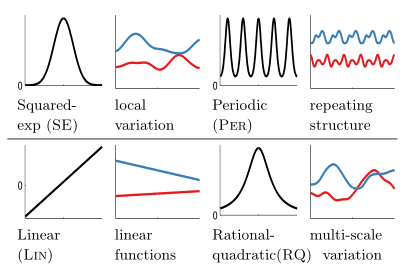
\includegraphics[width=0.6\textwidth]{base.png}
  \caption{base kernel及其描述的时间序列}\label{2}
\end{figure}

\begin{figure}
  \centering
  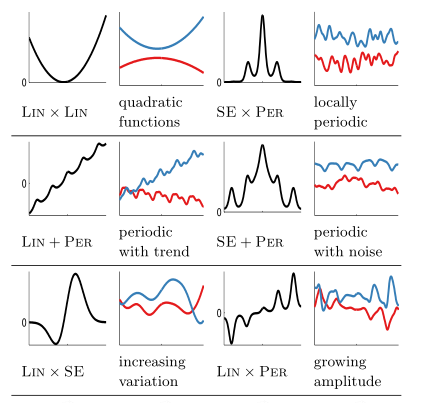
\includegraphics[width=0.6\textwidth]{com.png}
  \caption{Compositional Kernel及其描述的时间序列}\label{3}
\end{figure}

\begin{figure}
  \centering
  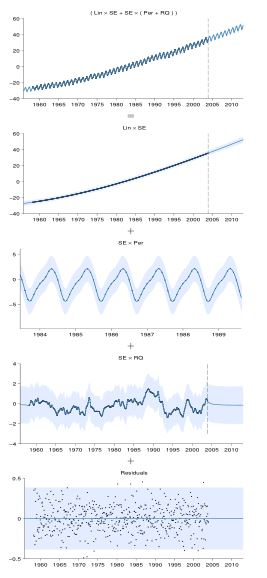
\includegraphics[width=0.5\textwidth]{kernel.jpg}
  \caption{Compositional Kernel分解示意图}\label{1}
\end{figure}

\end{enumerate}

\section*{下周计划}
\begin{itemize}
  \item 继续看GP kernel相关论文。还有时间的话了解机器学习其他领域知识。
\end{itemize}

\end{document} 